In this section we compare the Standard Model Higgs exclusion limits
for different channels.

\begin{figure}[!hbtp]

\centering
\subfigure[SF 0-Jet Cut]{
\centering
\label{subfig:sf_0j_cut}
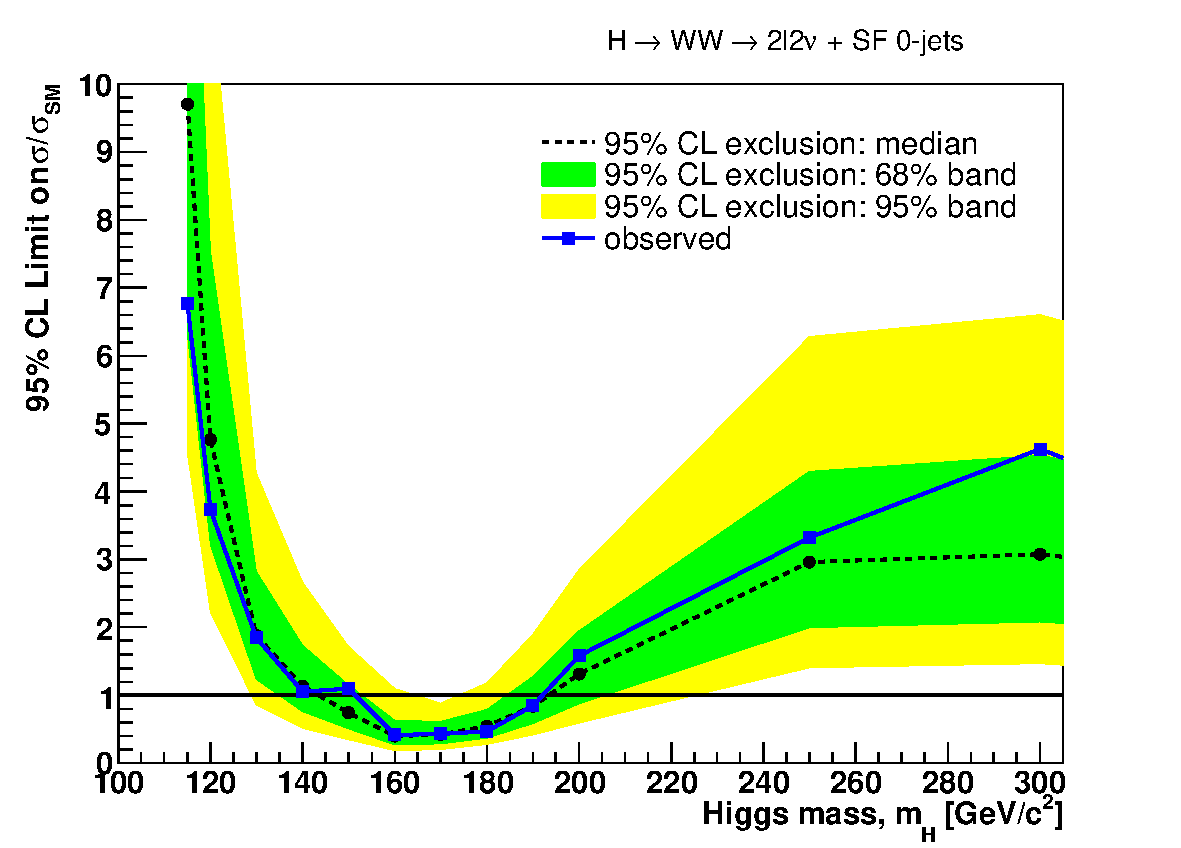
\includegraphics[width=.45\textwidth]{figures/limits_sf_0j_cut.pdf}}
\subfigure[OF 0-Jet Cut]{
\centering
\label{subfig:of_0j_cut}
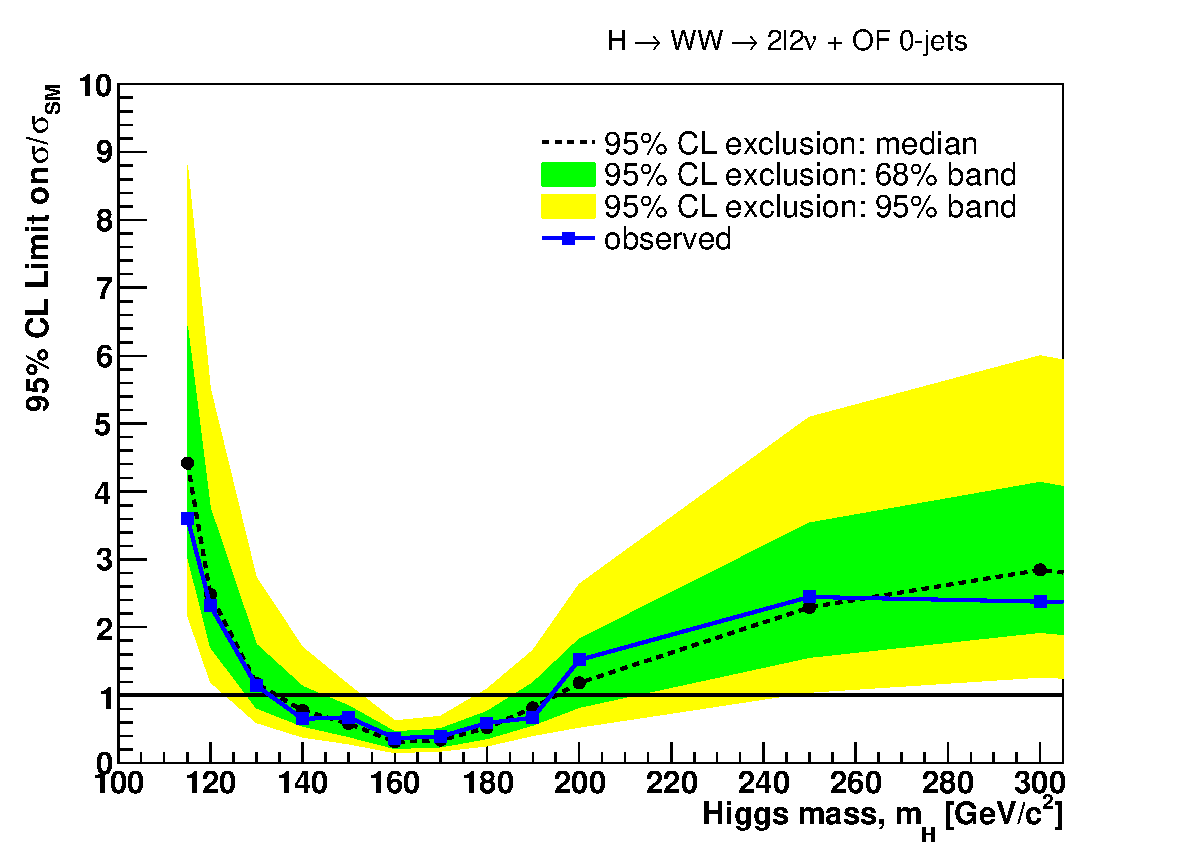
\includegraphics[width=.45\textwidth]{figures/limits_of_0j_cut.pdf}}
%% \subfigure[ee and $\mu\mu$ 0-Jet]{
%% \centering
%% \label{subfig:dyr_mh0_2j}
%% 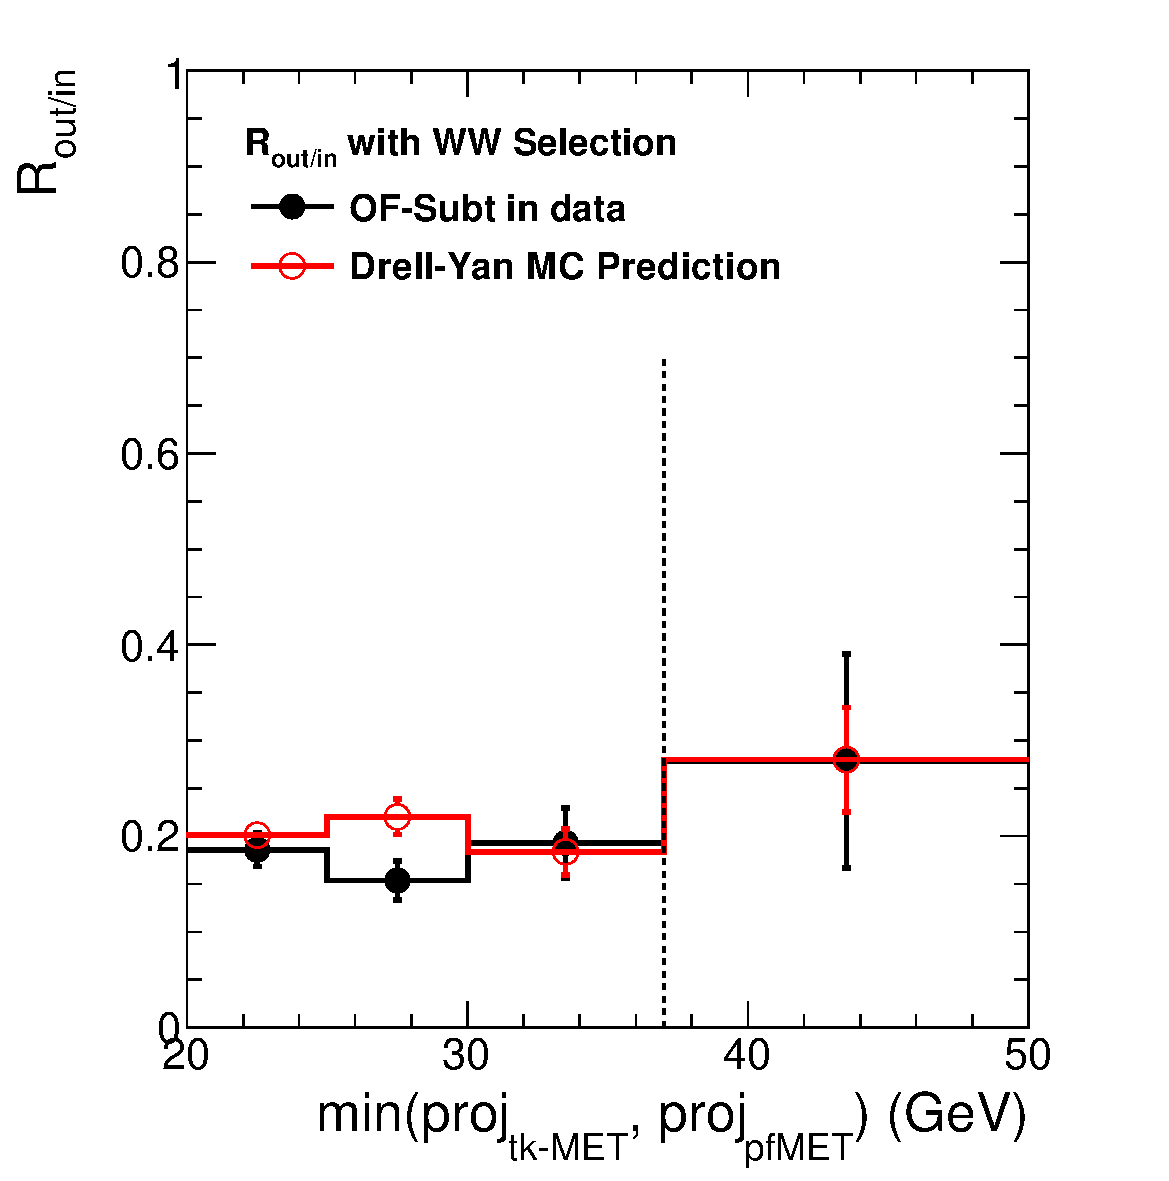
\includegraphics[width=.3\textwidth]{figures/Routin_0Jet_mH0_4000pb_dy.pdf}}
%% \centering
%% \subfigure[ee 1-Jet]{
%% \centering
%% \label{subfig:dyr_ee_mh0}
%% 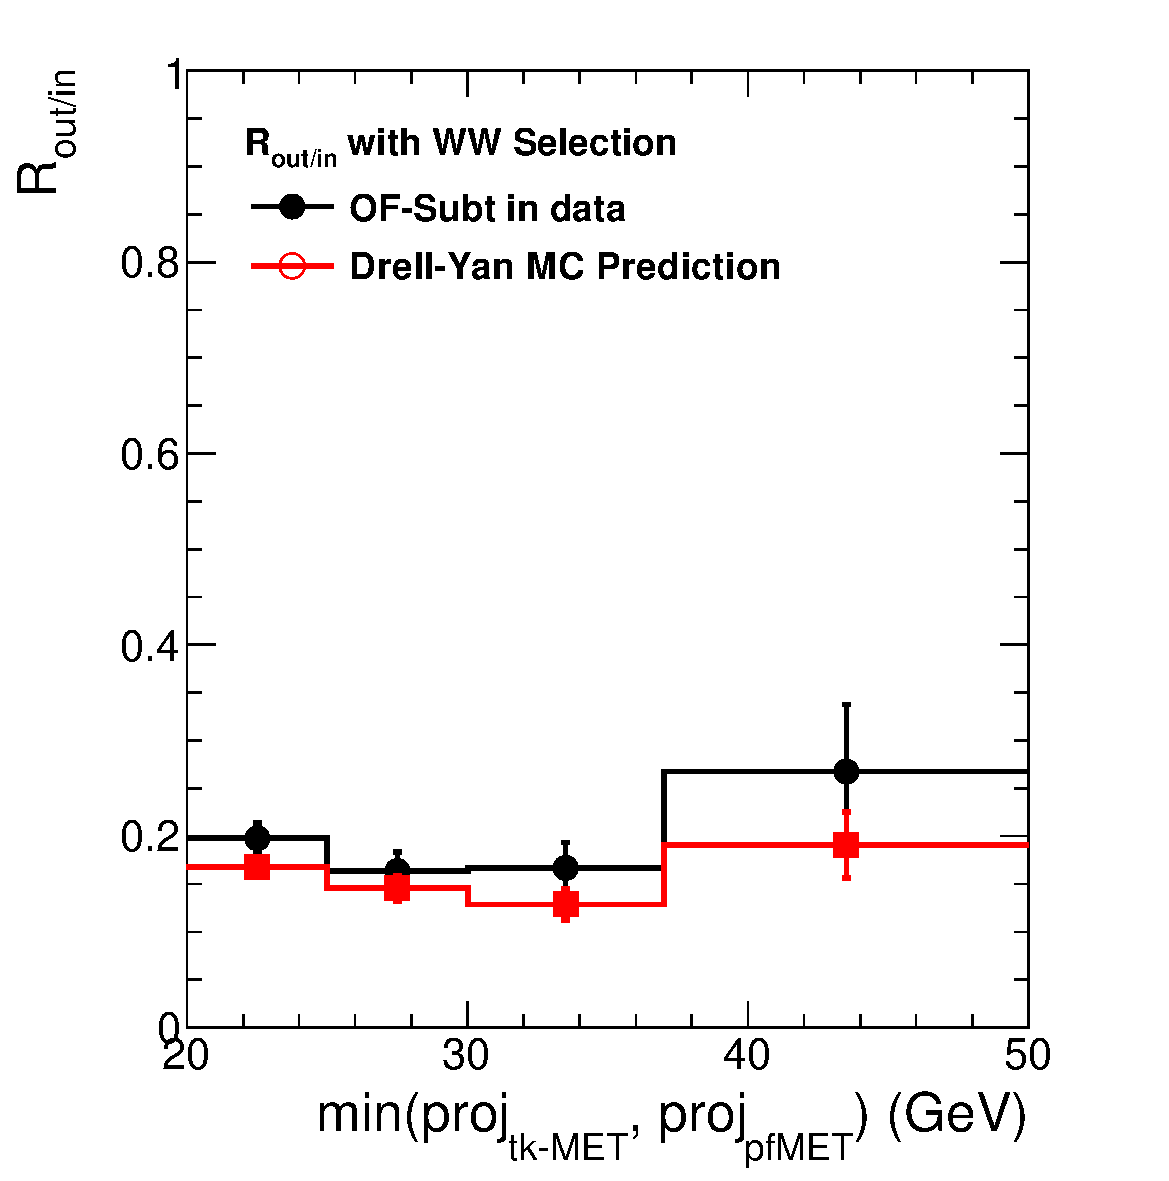
\includegraphics[width=.3\textwidth]{figures/Routin_ee_1Jet_mH0_4000pb_dy.pdf}}
%% \subfigure[$\mu\mu$ 1-Jet]{
%% \centering
%% \label{subfig:dyr_mm_mh0}
%% 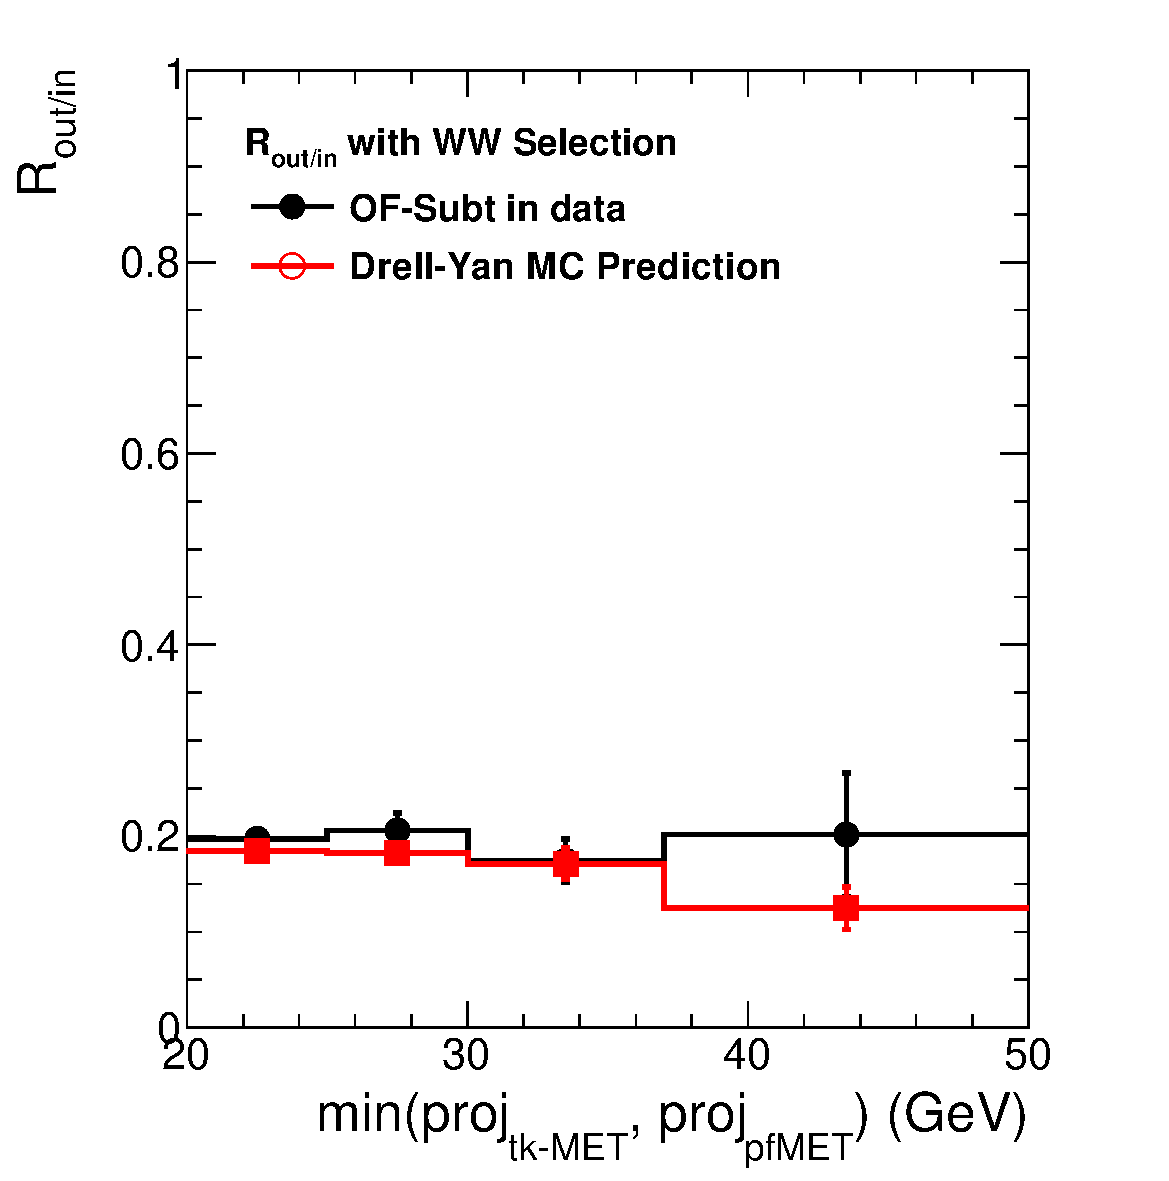
\includegraphics[width=.3\textwidth]{figures/Routin_mm_1Jet_mH0_4000pb_dy.pdf}}
%% \subfigure[ee and$\mu\mu$ 1-Jet]{
%% \centering
%% \label{subfig:dyr_mh0}
%% 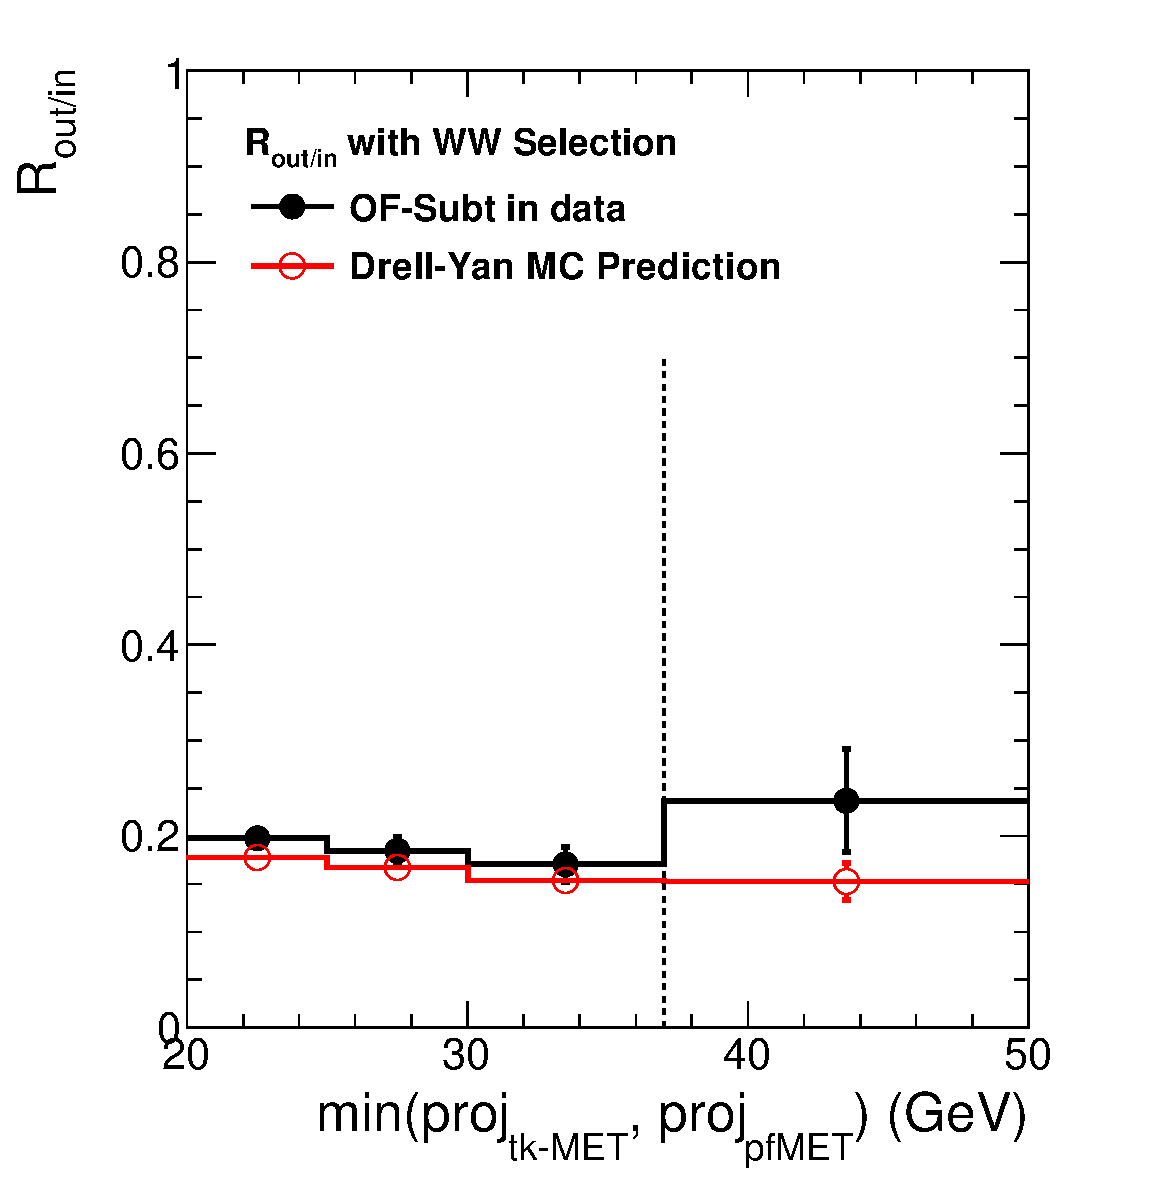
\includegraphics[width=.3\textwidth]{figures/Routin_1Jet_mH0_4000pb_dy.pdf}}
%% \subfigure[ee 2-Jet]{
%% \centering
%% \label{subfig:dyr_ee_mh0}
%% 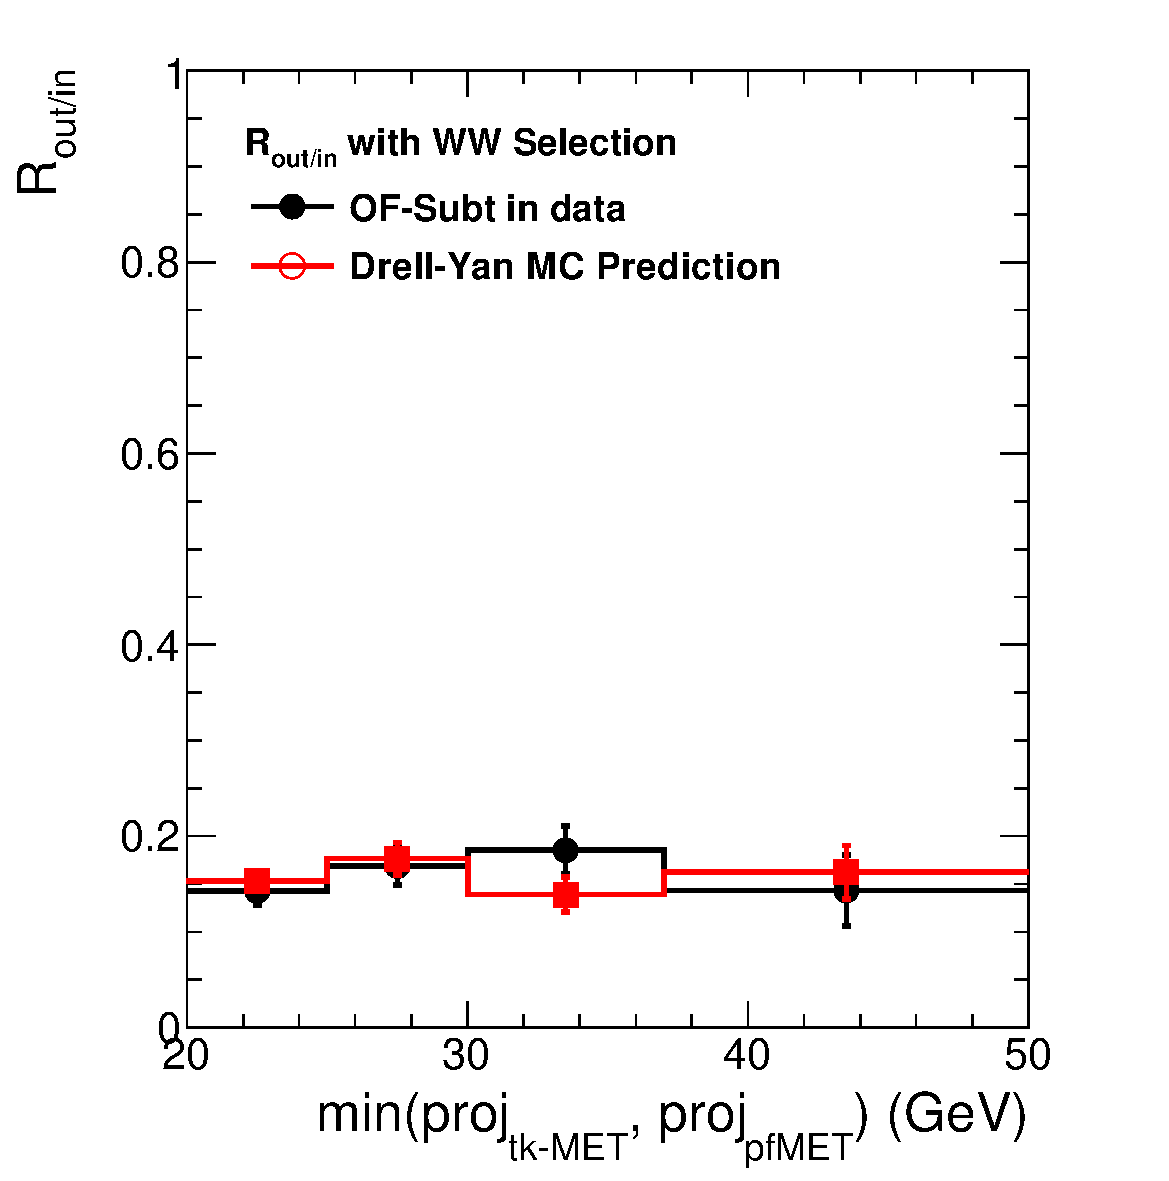
\includegraphics[width=.3\textwidth]{figures/Routin_ee_2Jet_mH0_4000pb_dy.pdf}}
%% \subfigure[$\mu\mu$ 2-Jet]{
%% \centering
%% \label{subfig:dyr_mm_mh0}
%% 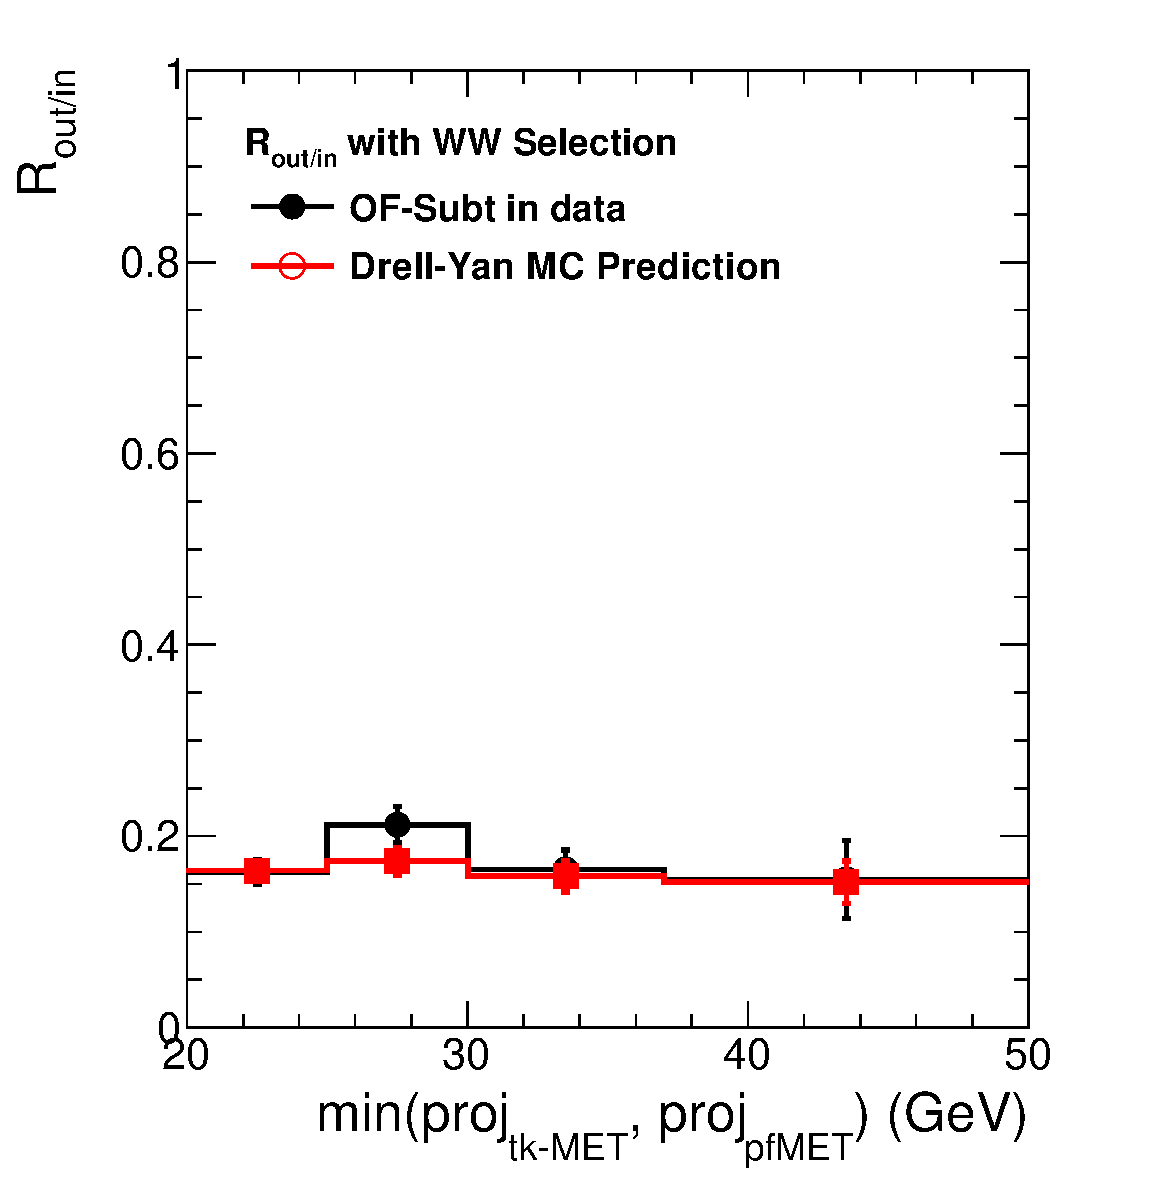
\includegraphics[width=.3\textwidth]{figures/Routin_mm_2Jet_mH0_4000pb_dy.pdf}}
%% \subfigure[ee and $\mu\mu$ 2-Jet]{
%% \centering
%% \label{subfig:dyr_mh0}
%% 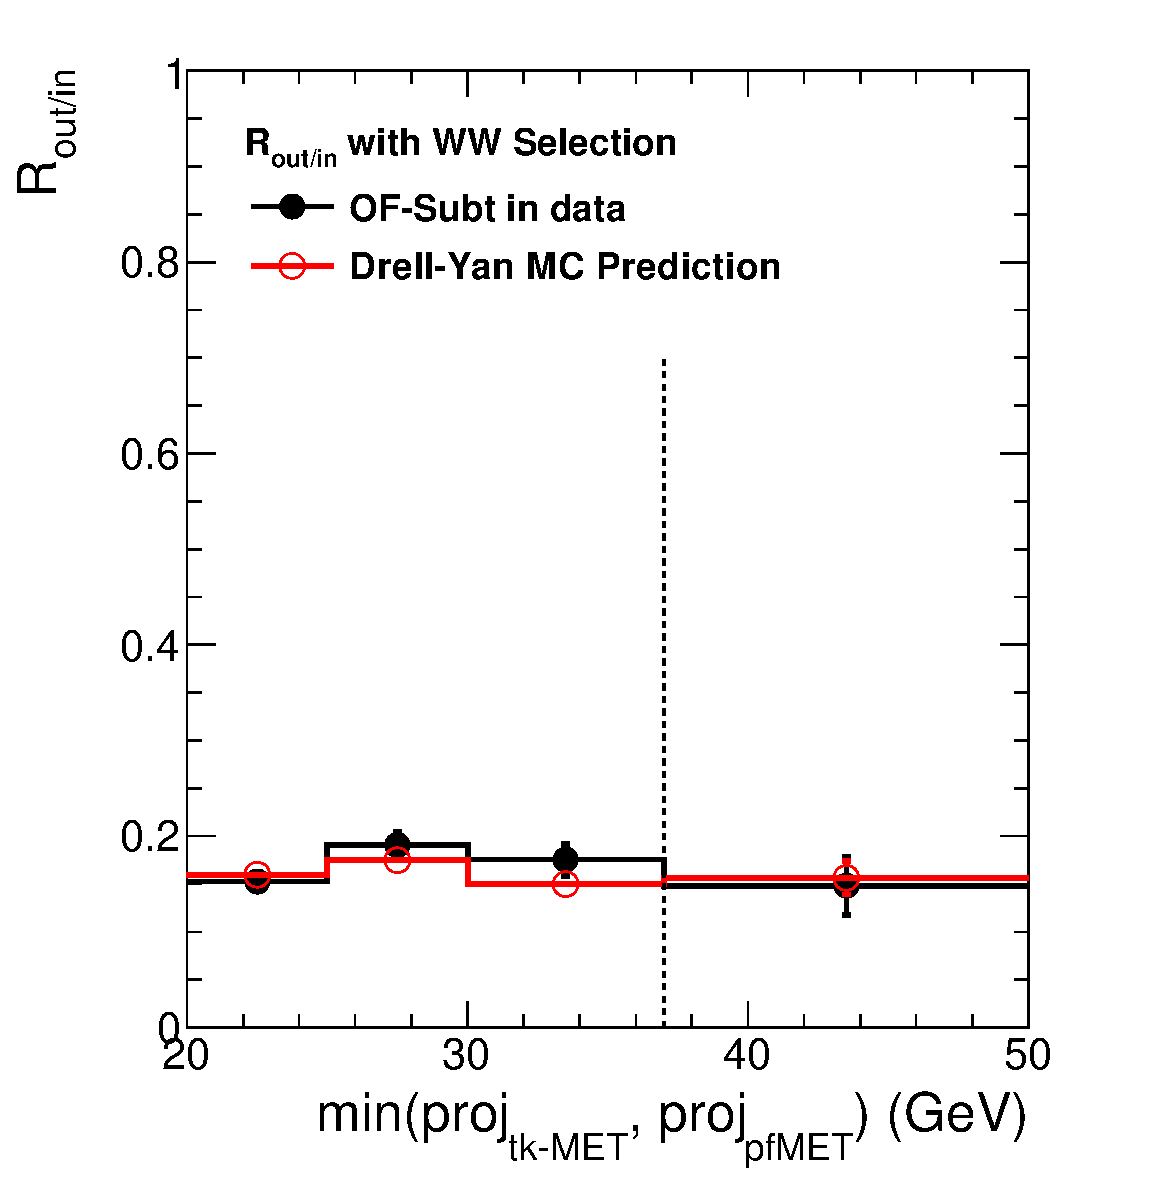
\includegraphics[width=.3\textwidth]{figures/Routin_2Jet_mH0_4000pb_dy.pdf}}
\caption{}
\label{fig:ul_cutbased_subchannels}
\end{figure}

%%%%%%%%%%%%%%%%%%%%%%%%%%%%%%
\begin{table}[!hbp]
\begin{center}
\begin{tabular}{c c c c c}
\hline
\vspace{-3mm} && \\
 Higgs Mass   & Observed & Median expected & Expected range for 68\% & Expected range for 95\%   \\
\vspace{-3mm} && \\
\hline
110 & 16.1 & 23.1 & [15.0, 36.8] & [10.8, 60.2] \\
115 & 6.8 & 9.7 & [6.3, 15.4] & [4.6, 25.3] \\
120 & 3.7 & 4.8 & [3.2, 7.5] & [2.2, 11.5] \\
130 & 1.9 & 1.9 & [1.2, 2.8] & [0.9, 4.3] \\
140 & 1.0 & 1.1 & [0.8, 1.7] & [0.5, 2.7] \\
150 & 1.1 & 0.7 & [0.5, 1.2] & [0.3, 1.7] \\
160 & 0.4 & 0.4 & [0.3, 0.6] & [0.2, 1.1] \\
170 & 0.4 & 0.4 & [0.3, 0.6] & [0.2, 0.9] \\
180 & 0.5 & 0.5 & [0.4, 0.8] & [0.3, 1.2] \\
190 & 0.8 & 0.8 & [0.6, 1.3] & [0.4, 1.9] \\
200 & 1.6 & 1.3 & [0.9, 1.9] & [0.6, 2.9] \\
250 & 3.3 & 3.0 & [2.0, 4.3] & [1.4, 6.3] \\
300 & 4.6 & 3.1 & [2.1, 4.5] & [1.5, 6.6] \\
350 & 3.3 & 2.7 & [1.9, 3.9] & [1.2, 5.7] \\
400 & 3.2 & 2.9 & [2.1, 4.3] & [1.4, 6.5] \\
450 & 4.2 & 4.1 & [2.8, 6.2] & [2.1, 8.9] \\
500 & 7.4 & 5.9 & [4.2, 8.6] & [3.1, 12.6] \\
550 & 15.4 & 9.0 & [6.3, 13.8] & [4.7, 19.8] \\
600 & 18.6 & 14.1 & [9.7, 20.4] & [7.3, 30.3] \\
\hline
\end{tabular}
\caption{Cut-based 0-jet same-flavor analysis. Expected and observed
  upper limits for \intlumi\ of data}
\label{tab:sf0_cut}
\end{center}
\end{table}
%%%%%%%%%%%%%%%%%%%%%%%%%%%%%%

%%%%%%%%%%%%%%%%%%%%%%%%%%%%%%
\begin{table}[!hbp]
\begin{center}
\begin{tabular}{c c c c c}
\hline
\vspace{-3mm} && \\
 Higgs Mass   & Observed & Median expected & Expected range for 68\% & Expected range for 95\%   \\
\vspace{-3mm} && \\
\hline
110 & 7.4 & 9.1 & [6.3, 13.2] & [4.5, 18.1] \\
115 & 3.6 & 4.4 & [3.0, 6.4] & [2.2, 8.8] \\
120 & 2.3 & 2.5 & [1.7, 3.8] & [1.2, 5.5] \\
130 & 1.1 & 1.2 & [0.8, 1.7] & [0.6, 2.7] \\
140 & 0.7 & 0.8 & [0.5, 1.1] & [0.4, 1.7] \\
150 & 0.7 & 0.6 & [0.4, 0.8] & [0.3, 1.2] \\
160 & 0.4 & 0.3 & [0.2, 0.5] & [0.2, 0.6] \\
170 & 0.4 & 0.3 & [0.2, 0.5] & [0.2, 0.7] \\
180 & 0.6 & 0.5 & [0.4, 0.8] & [0.3, 1.1] \\
190 & 0.7 & 0.8 & [0.6, 1.2] & [0.4, 1.7] \\
200 & 1.5 & 1.2 & [0.8, 1.8] & [0.5, 2.6] \\
250 & 2.4 & 2.3 & [1.6, 3.5] & [1.0, 5.1] \\
300 & 2.4 & 2.8 & [1.9, 4.1] & [1.3, 6.0] \\
350 & 2.3 & 2.5 & [1.6, 3.5] & [1.2, 5.4] \\
400 & 2.8 & 2.7 & [1.8, 4.1] & [1.3, 5.9] \\
450 & 3.7 & 3.5 & [2.4, 5.4] & [1.7, 8.1] \\
500 & 4.1 & 5.3 & [3.6, 7.4] & [2.6, 10.7] \\
550 & 6.7 & 7.8 & [5.4, 12.2] & [3.8, 17.8] \\
600 & 12.6 & 11.7 & [8.1, 18.6] & [5.7, 27.1] \\
\hline
\end{tabular}
\caption{Cut-based 0-jet opposite-flavor analysis. Expected and observed
  upper limits for \intlumi\ of data}
\label{tab:sf0_cut}
\end{center}
\end{table}
%%%%%%%%%%%%%%%%%%%%%%%%%%%%%%
